Para la construcción del nodo 1, usaremos el siguiente cableado de la placa
Arduino Pro Mini:

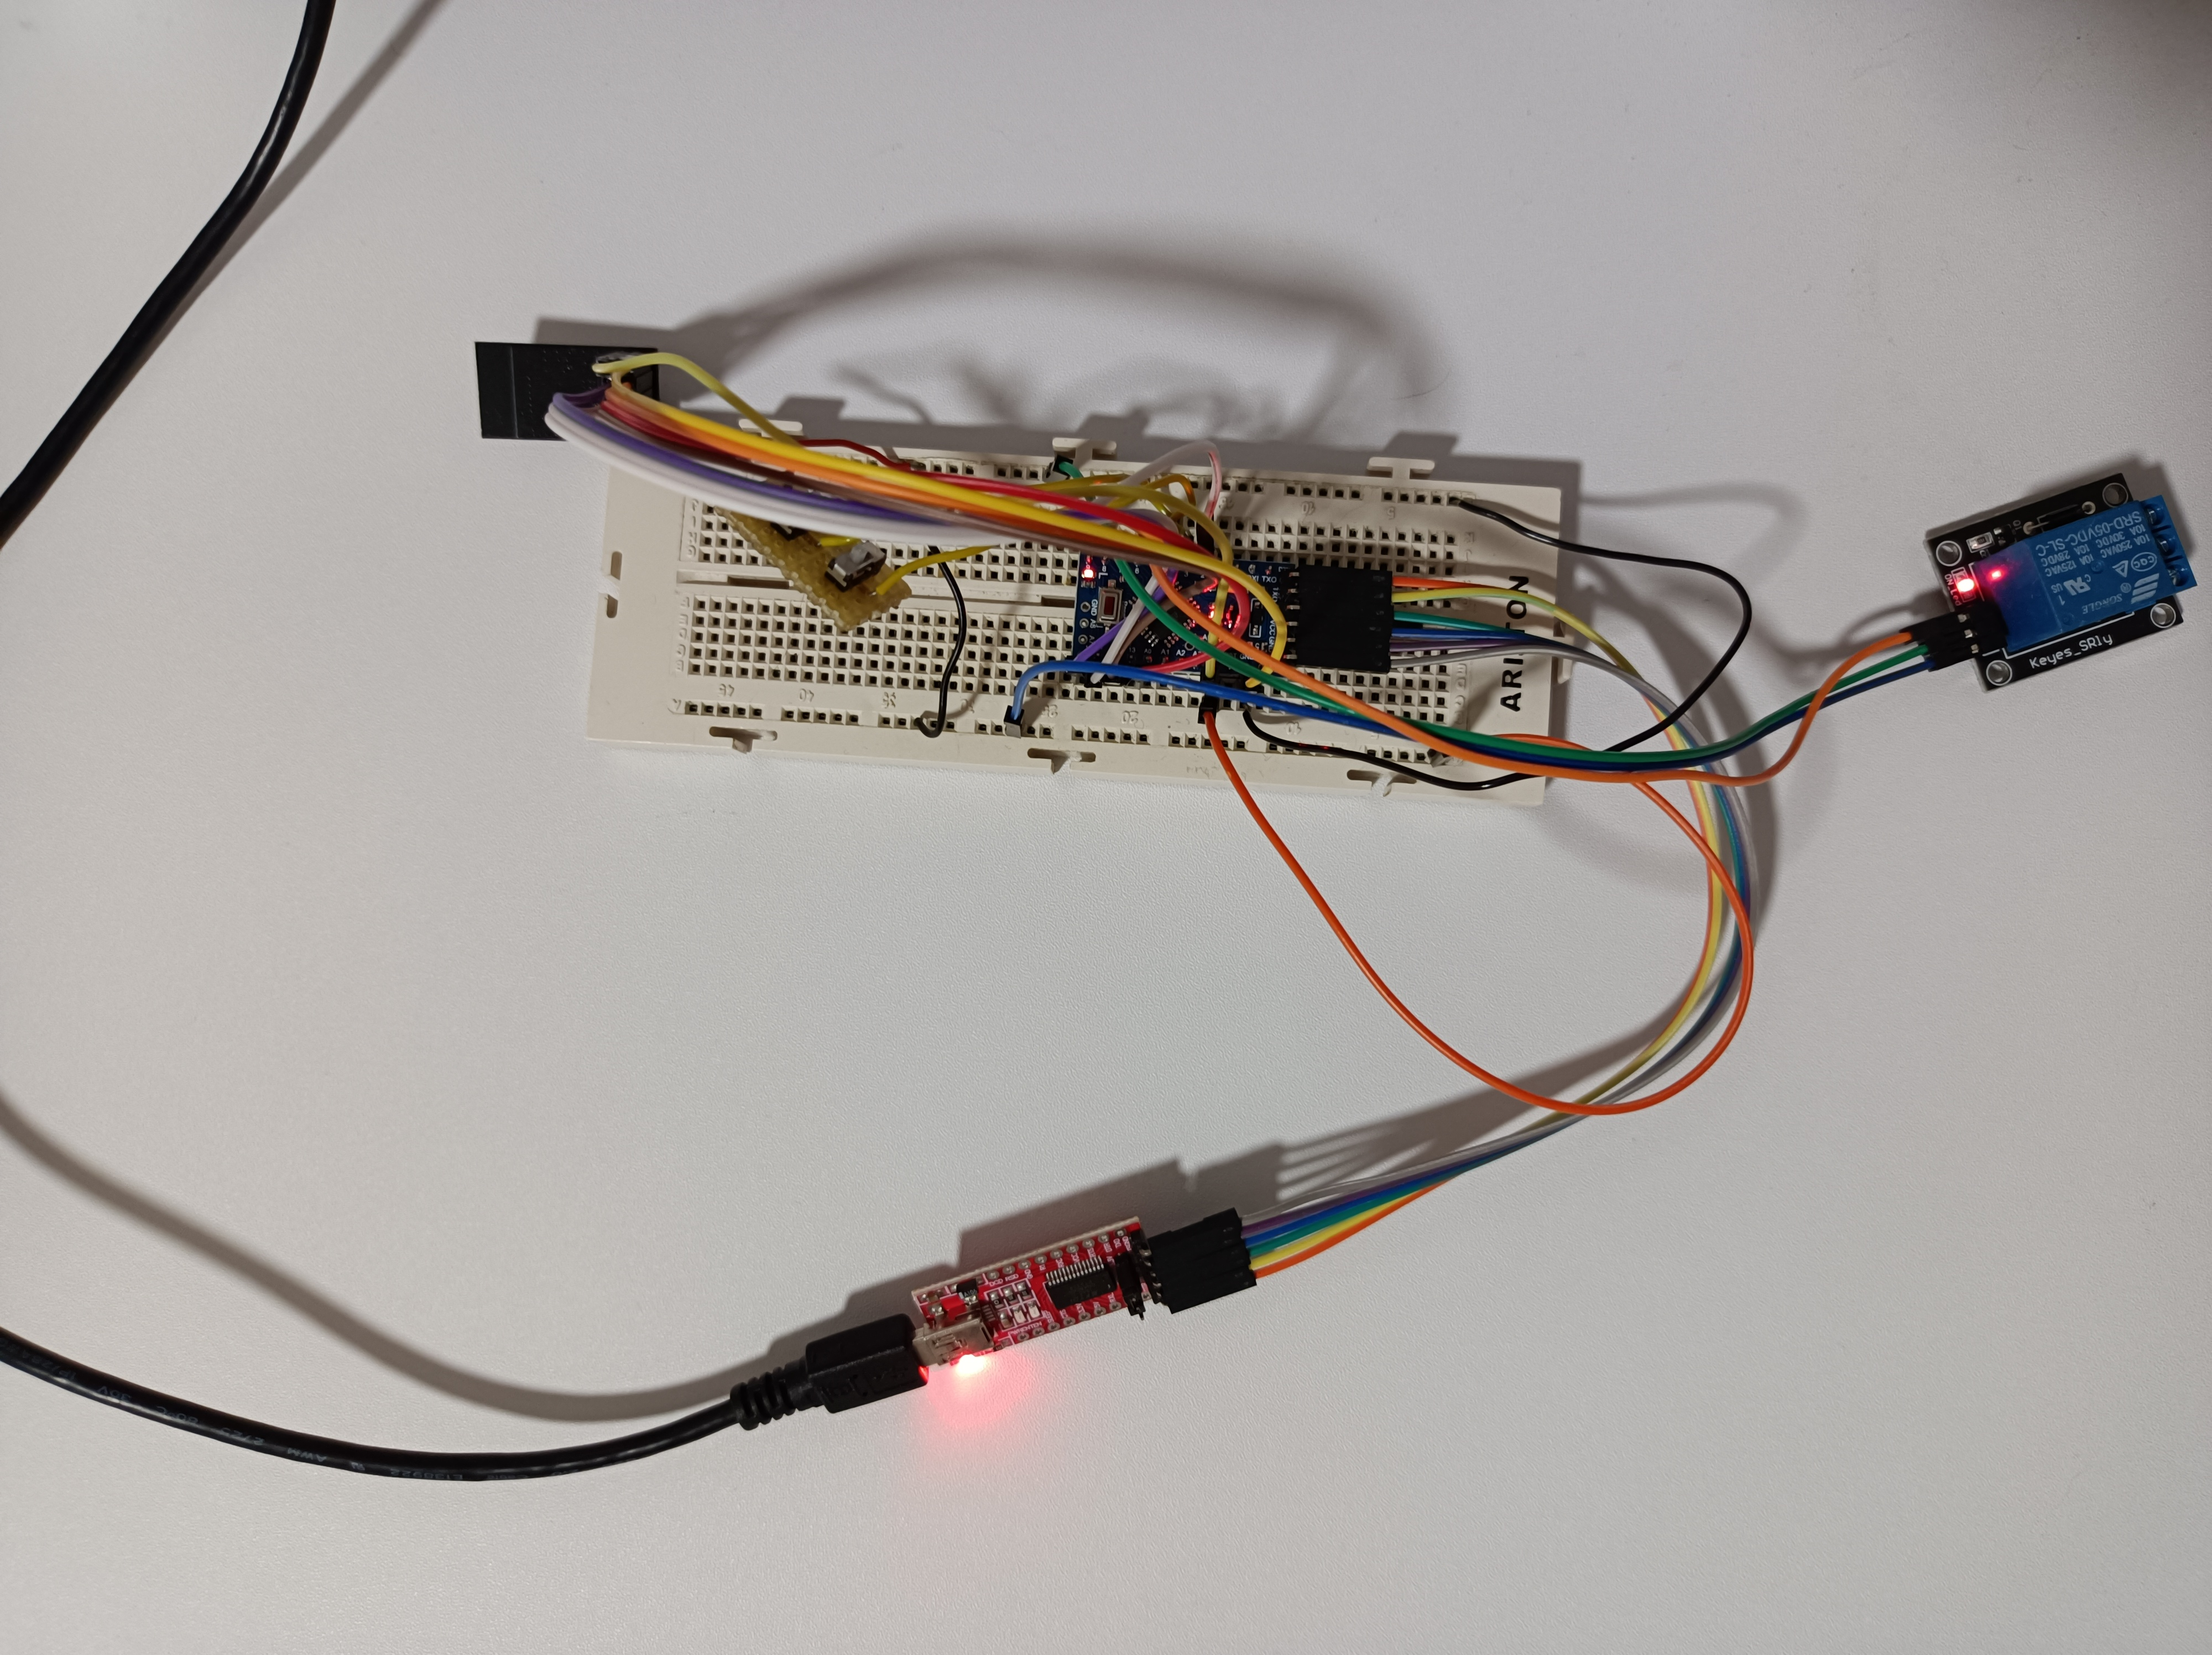
\includegraphics[width=\linewidth]{nodo1/nodo1-wiring.jpg}

La conexión del transmisor de radio NRF24L01 sigue el siguiente esquema:

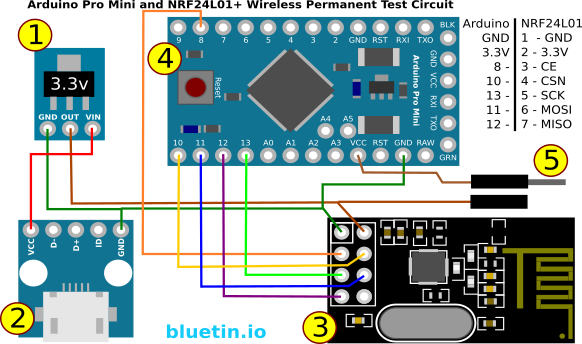
\includegraphics[width=\linewidth]{arduino-nrf24l01-wiring.jpg}

Y a la Raspberry Pi también se le conecta otro transmisor igual:

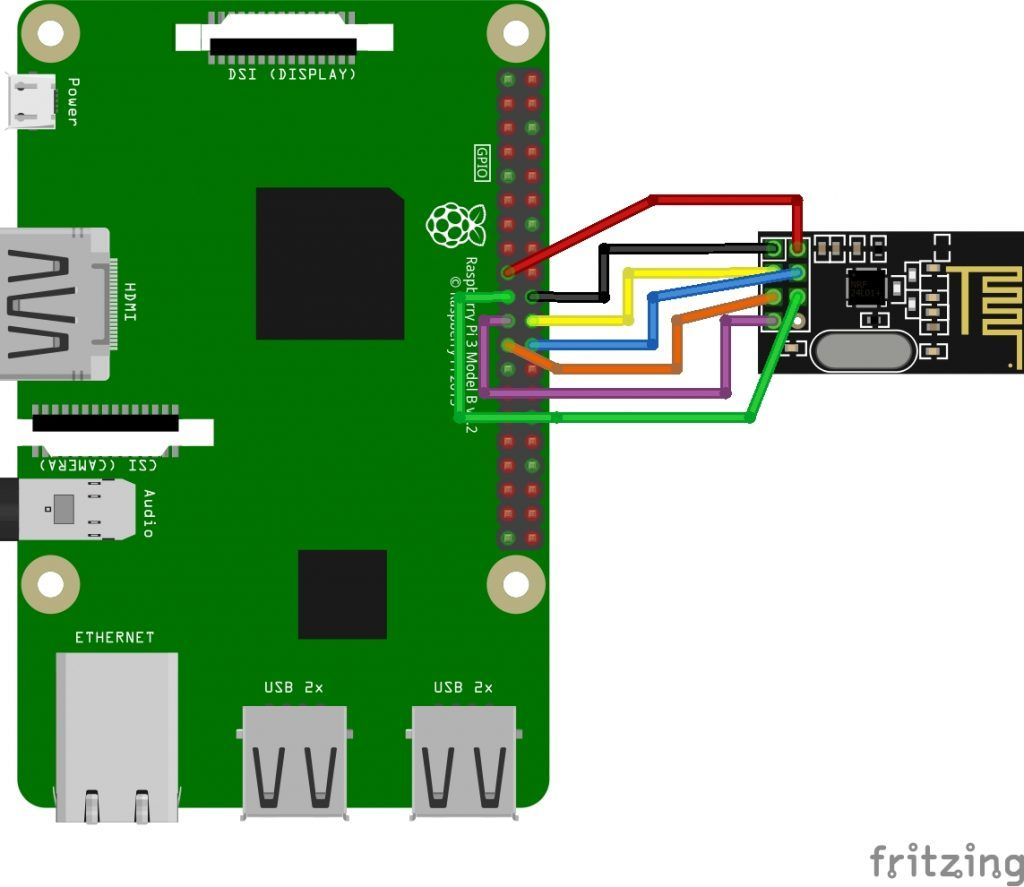
\includegraphics[width=\linewidth]{rpi-nrf24l01-wiring.jpg}

Para la programación de la placa, hay que descargar la librería
\emph{MySensors}, versión \emph{2.3.2}\footnotemark. Para el nodo 1 en
particular, también usaremos la librería \emph{Bounce2}, versión
\emph{2.71.0}\footnotemark.

\footnotetext{\url{
    https://github.com/mysensors/MySensors/archive/refs/tags/2.3.2.zip
}}
\footnotetext{\url{
    https://github.com/thomasfredericks/Bounce2/archive/refs/tags/v2.71.zip
}}

El código que usaremos es el que procede:

\lstinputlisting[language=C++, caption=nodo1.ino]{2/nodo1/nodo1.ino}

Al programar la placa para ambos ejercicios de este bloque hay que tener
cuidado de que el IDE tenga seleccionado el procesador correcto en
\emph{Tools $\rightarrow$ Processor} en el menú superior, que en nuestro caso
es el \emph{ATmega328P (3.3V, 8 MHz)}, tal y como se indica en la imagen:

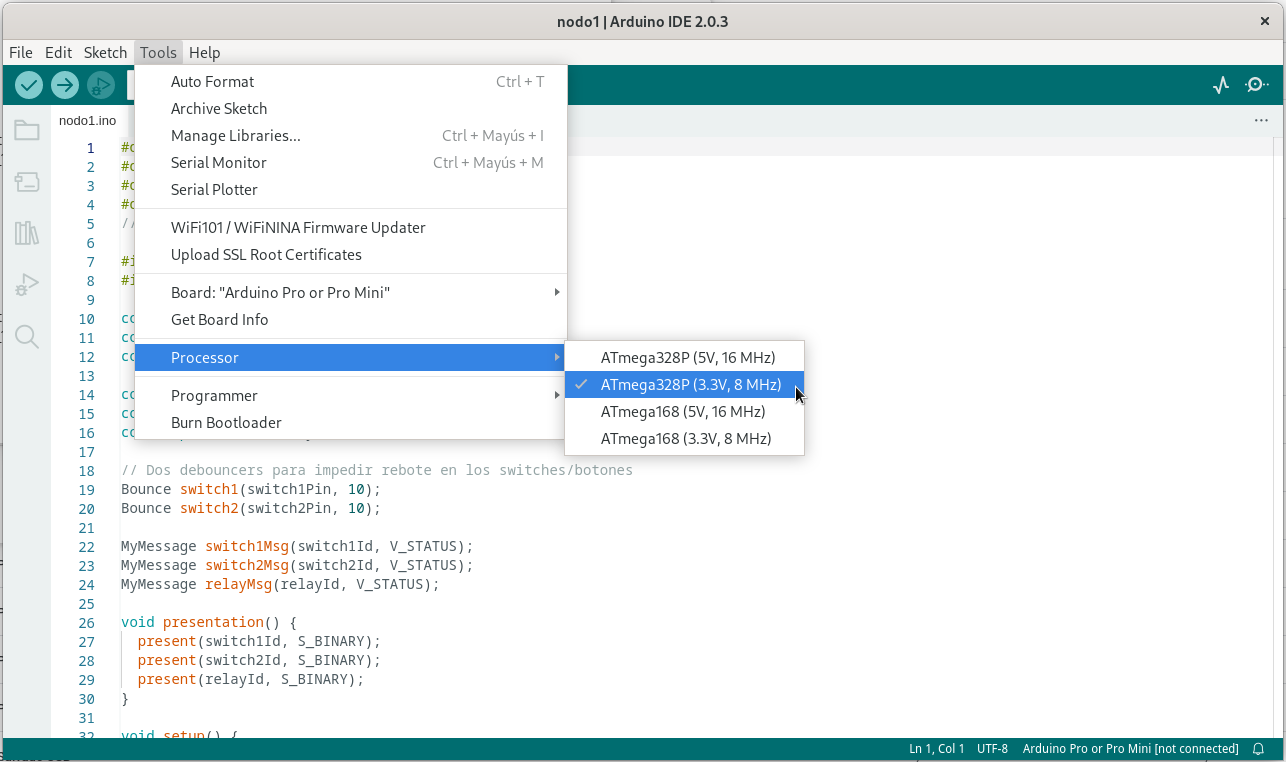
\includegraphics[width=\linewidth]{arduino-ide-processor.png}

Finalmente, en el menú \emph{Configuración $\rightarrow$ Dispositivos} de
Domoticz deberían salir tres entradas como las siguientes, pudiendo activar y
desactivar el relé, que se corresponde con el ID de dispositivo 3:

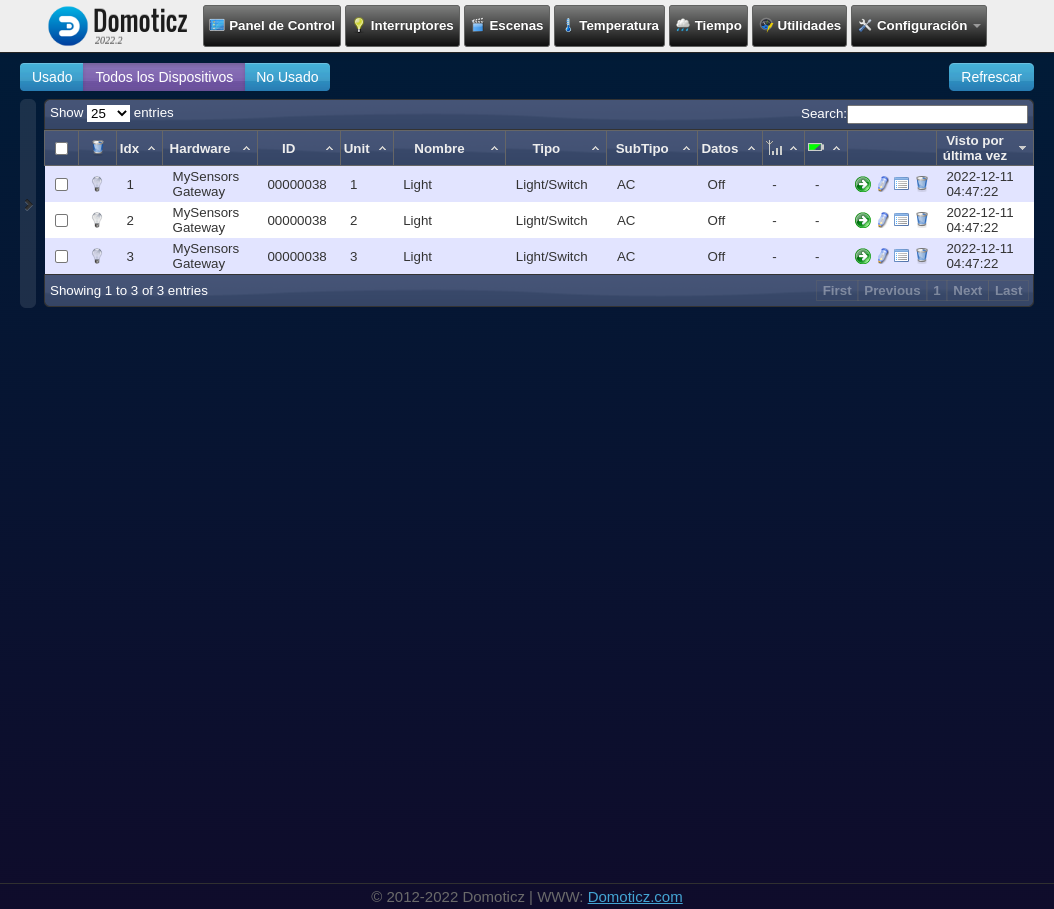
\includegraphics[width=\linewidth]{nodo1/nodo1-domoticz.png}